\documentclass[12pt]{article}

\usepackage[utf8]{inputenc}
\usepackage{graphicx}
\usepackage[portuguese]{babel}
\usepackage{float}

\title{MAC0344 Arquitetura de Computadores\\
Lista de Exercícios No. 1
}
\author{Mateus Agostinho dos Anjos\\NUSP 9298191}
\date{\today}

\begin{document}
	\maketitle
	\begin{itemize}
		\item[1 -]
			Na lista top500 de junho deste ano (2019), os
			computadores instalados no Brasil são:\\
			\begin{table}[h]
				\begin{tabular}{c|c|c|c}
					\textbf{Nome no TOP500} & \textbf{Número de \textit{Cores}} & \textbf{Vel. Linpack} & \textbf{Vel. de Pico}\\
					Petróleo Brasileiro S.A & 48,384 & 1,836 TFlop/s & 4,297.42 TFlop/s\\
					Cloud Provider & 38,400 & 1,123.15 TFlop/s & 1,413.12 TFlop/s\\
					Software Company (M) & 38,400 & 1,123.15 TFlop/s& 1,413.12 TFlop/s\\
				\end{tabular}
			\end{table}
					\begin{table}[h]
				\begin{tabular}{c|c|c}
					\textbf{Nome no TOP500} & \textbf{Número de Classificação (06/2019)} & \textbf{Localização}\\
					Petróleo Brasileiro S.A & 142 & Rio de Janeiro\\
					Cloud Provider & 418 & Não Informado\\
					Software Company (M) & 429 & Não Informado\\
				\end{tabular}
			\end{table}
			\newpage	
		\item[2 -]
			Veremos alguns gráficos que mostram a evolução de performance
			entre Processadores e Memória
			\hfill\newline
			\begin{minipage}{\linewidth}
				\centering
  				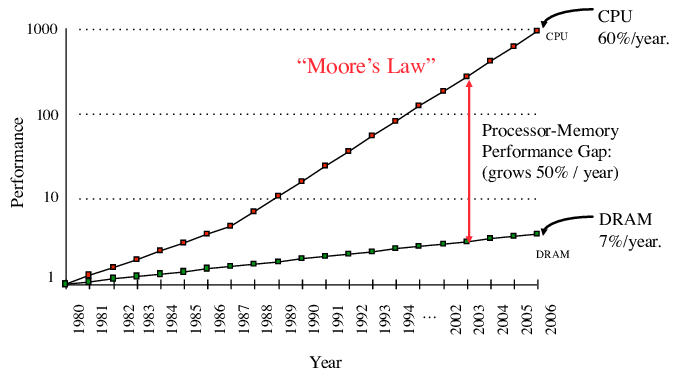
\includegraphics[width=12cm]{Memory-Access-vs-CPU-Speed.png}
  				\newline
  				Primeiro Exemplo até 2006
			\end{minipage}
			\hfill\newline\newline\newline\newline
			\begin{minipage}{\linewidth}
				\centering
  				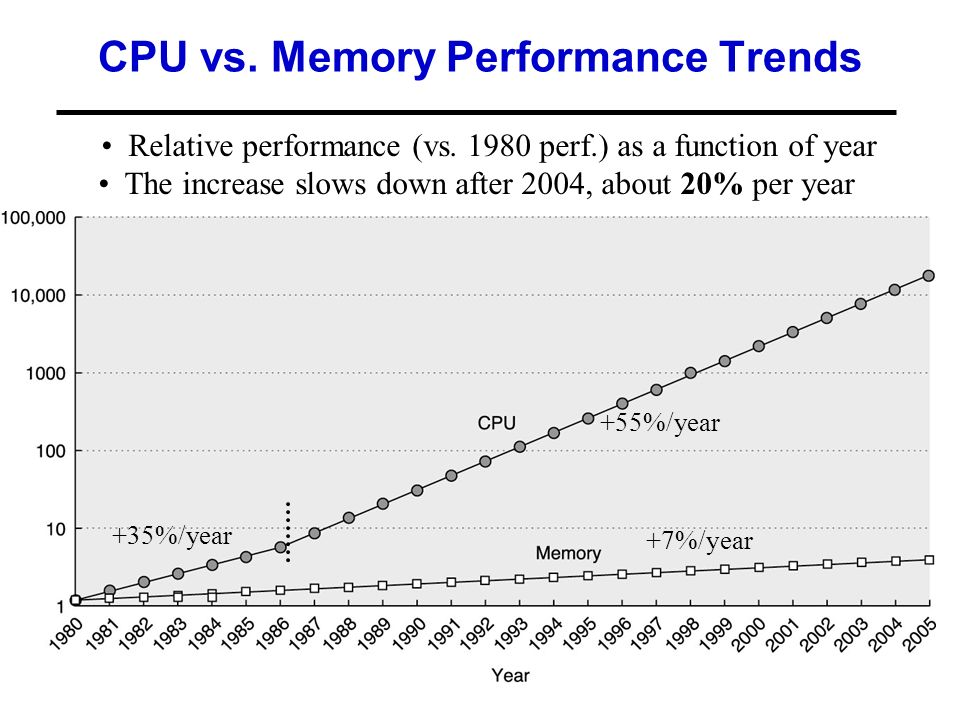
\includegraphics[width=12cm]{CPU-vs-Memory-Trends.jpg}
  				\newline
  				Segundo Exemplo explicitando período de 1995-2002
			\end{minipage}
			\hfill\newline
			\begin{minipage}{\linewidth}
				\centering
  				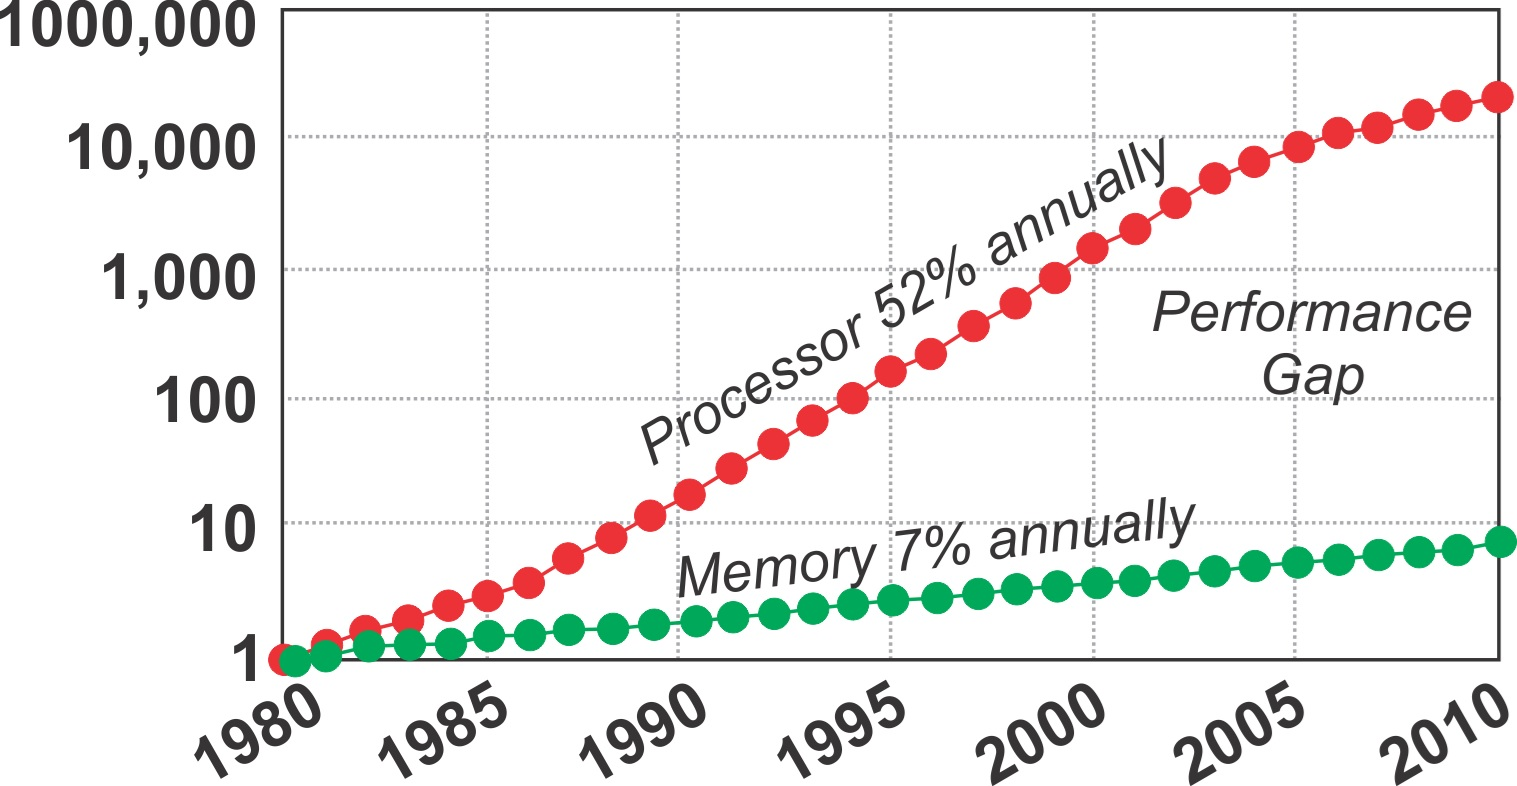
\includegraphics[width=12cm]{CPU-vs-Memory-Colorized.jpg}
  				\newline
  				Terceiro Exemplo até o ano de 2010
			\end{minipage}
			\hfill\newline\newline
			Os exemplos acima nos mostram que \textbf{a performance dos 
			processadores avança mais rápido do que a performance
			das memórias}. Percebemos tal fenômeno a partir das diferentes
			angulações que as retas apresentam (mesmo variando ligeiramente
			de gráfico para gráfico), aumentando o "gap" entre
			elas.
	\end{itemize}
		
\end{document}